%\documentclass[10pt,notes]{beamer}       % print frame + notes
%\documentclass[10pt, notes=only]{beamer}   % only notes
\documentclass[11pt]{beamer}              % only frames

%%%%%% IF YOU WOULD LIKE TO CREATE LECTURE NOTES COMMENT OUT THE FOlLOWING TWO LINES
%\usepackage{pgfpages}
%\setbeameroption{show notes on second screen=bottom} % Both

\usepackage{graphicx}
\DeclareGraphicsExtensions{.pdf,.png,.jpg}
\usepackage{color}
\usetheme{winslab}
\usepackage[utf8]{inputenc}
\usepackage[english]{babel}
\usepackage{amsmath}
\usepackage{amsfonts}
\usepackage{amssymb}




\usepackage{algorithm2e,algorithmicx,algpseudocode}
\algnewcommand\Input{\item[\textbf{Input:}]}%
\algnewcommand\Output{\item[\textbf{Output:}]}%
\newcommand\tab[1][1cm]{\hspace*{#1}}

\algnewcommand{\Implement}[2]{\item[\textbf{Implements:}] #1 \textbf{Instance}: #2}%
\algnewcommand{\Use}[2]{\item[\textbf{Uses:}] #1 \textbf{Instance}: #2}%
\algnewcommand{\Trigger}[1]{\Statex{\textbf{Trigger:} (#1)}}%
\algnewcommand{\Events}[1]{\item[\textbf{Events:}] #1}%
\algnewcommand{\Need}[1]{\item[\textbf{Needs:}] #1}%
\algnewcommand{\Event}[2]{\Statex \item[\textbf{On#1:}](#2) \textbf{do}}%
\algnewcommand{\Trig}[3]{\State \textbf{Trigger}  #1.#2 (#3) }%
\def\true{\textbf{T}}
\def\false{\textbf{F}}


\author[Ersel Hengirmen]{Ersel Hengirmen\\\href{mailto:ehengirmen@hotmail.com}{ehengirmen@hotmail.com}}
%\author[J.\,Doe \& J.\,Doe]
%{%
%  \texorpdfstring{
%    \begin{columns}%[onlytextwidth]
%      \column{.45\linewidth}
%      \centering
%      John Doe\\
%      \href{mailto:john@example.com}{john@example.com}
%      \column{.45\linewidth}
%      \centering
%      Jane Doe\\
%      \href{mailto:jane.doe@example.com}{jane.doe@example.com}
%    \end{columns}
%  }
%  {John Doe \& Jane Doe}
%}

\title[WINS Beamer Template]{Leader Election in IEEE 1394}
%\date{} 

\begin{document}

\begin{frame}[plain]
\titlepage
\note{In this talk, I will present .... Please answer the following questions:
\begin{enumerate}
\item Why are you giving presentation?
\item What is your desired outcome?
\item What does the audience already know  about your topic?
\item What are their interests?
\item What are key points?
\end{enumerate}
}
\end{frame}

\begin{frame}[label=toc]
    \frametitle{Outline of the Presentation}
    \tableofcontents[subsubsectionstyle=hide]
\note{ The possible outline of a talk can be as follows.
\begin{enumerate}
\item Outline 
\item Problem and background
\item Design and methods
\item Major findings
\item Conclusion and recommendations 
\end{enumerate} Please select meaningful section headings that represent the content rather than generic terms such as ``the problem''. Employ top-down structure: from general to more specific.
}
\end{frame}
%
%\part{This the First Part of the Presentation}
%\begin{frame}
%        \partpage
%\end{frame}
%
\section{The Problem}
%\begin{frame}
%        \sectionpage
%\end{frame}

\begin{frame}{The problem}
    \begin{block}{Leader Election} 
        IEEE 1394, also known as FireWire is a standard for high-speed serial bus comminication.
        It is commonly used in audio and video equipment.
        In such networks devices are hot-pluggable, meaning they can be added or removed at any time without disrupting the system's operation.
        However, such changes trigger a bus reset, and after the reset, all nodes within the network are restored to an equal status, requiring a new leader to be elected dynamically.
    \end{block}
\end{frame}

\section{The Contribution}
\begin{frame}
\frametitle{What is the solution/contribution}
    \framesubtitle{}
	\begin{itemize}
		\item Implementation of Leader Election Algorithm on the AHCv2 platform.
		\item Anlysis of the algorithms within different topologies
	\end{itemize}
\end{frame}


\section{Motivation/Importance}
\begin{frame}
\frametitle{Motivation/Importance - 1}
The bus resets that happen after an audio or video plug-in can be disruptive, causing interruptions in the system's operation. Think as when you are on your computer watching a video you unplug your headphone and your system freezes for 3-4 seconds. That is not a situation anyone wants. 
\end{frame}
\begin{frame}
\frametitle{Motivation/Importance - 2}
The IEEE 1394 leader election protocol dynamically assigns leadership status after bus resets, the protocol creates uninterrupted communication and coordination among interconnected devices. This is crucial for the seamless exchange of digitized video and audio signals in various electronic devices.
\end{frame}



\section{Background/Previous Works}

\subsection{Background, Previous Works}
\begin{frame}{Background-1}
	The IEEE 1394 standard mentions about the problem under the concept of isochronous resource manager (IRM) selection.
	It also provides examples of processes for selecting the IRM within a backplane environment.
	However, it doesn't go into the algorithmic details of how the selection process should be implemented.
\end{frame}
\begin{frame}{Background-2}
	Additionally, Devillers et al., formalizes a simple algorithm for this IEEE standard protocol.
	This paper addresses ambiguities and challenges encountered during the process.
	The authors of the paperesspecially focuses on the tree identify phase.
	This paper serves as formal verification of this distributed algorithm. We will also use their method in our implementation.
\end{frame}




\section{Contribution}
\begin{frame}
	\frametitle{Protocol}
    The protocol operates in a decentralized manner where nodes in the network coordinate to form a tree structure. When a node has received a parent request from all but one of its neighbors it sends a parent request to its remaining neighbor. If a node has received parent requests from all its neighbors, it
    knows that it is has been elected as the root of the tree. There are 3 main states for every node of the algorihtm
\end{frame}


\subsection{Algorithm}

\begin{frame}
\frametitle{Algorithm-1}
\framesubtitle{Leader Election in IEEE 1394}
\begin{figure}
    \centering
    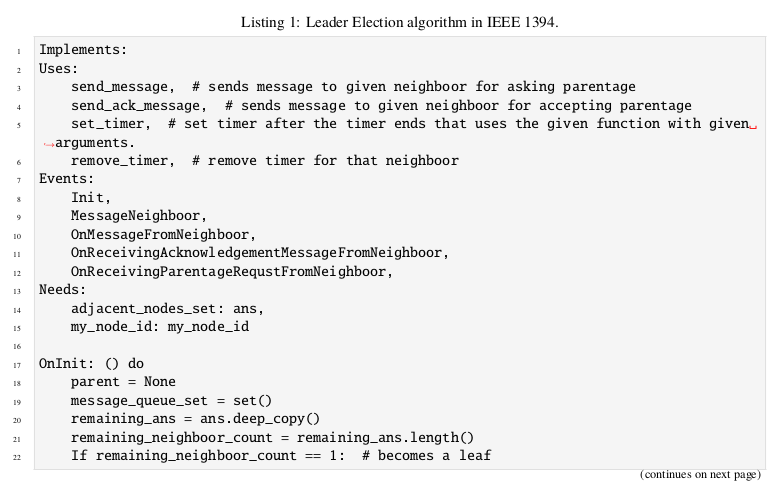
\includegraphics[scale=0.4]{figures/IEEE-1.png}
\end{figure}
\end{frame}

\begin{frame}
    \frametitle{Algorithm-2}
    \begin{figure}
        \centering
        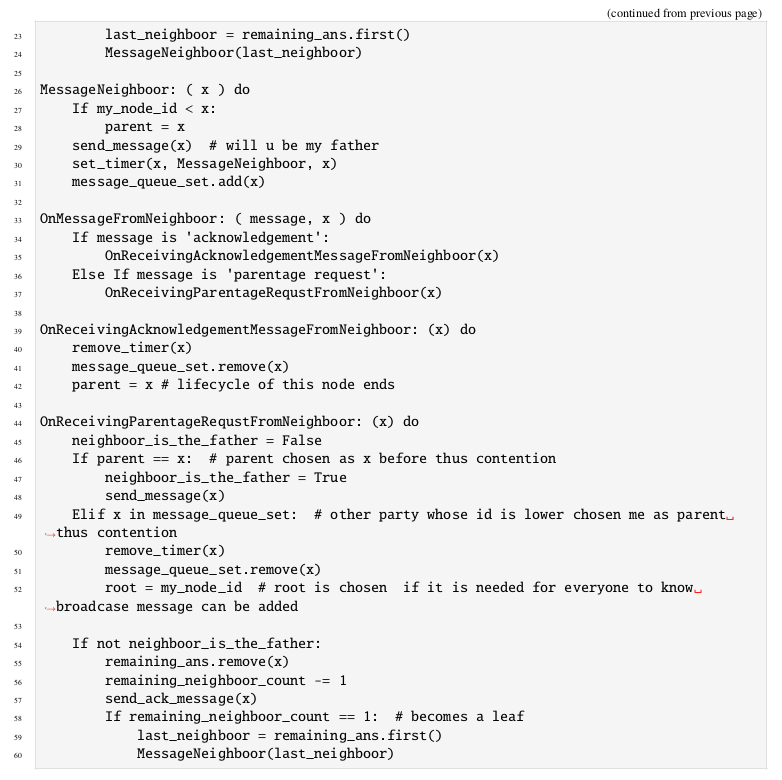
\includegraphics[scale=0.25]{figures/IEEE-2.png}
    \end{figure}
\end{frame}

\begin{frame}
\frametitle{States}


\begin{itemize}
	\item Waiting for Children
	\item Sending Parent Request
	\item Parent Contention(only for last 2 nodes)
\end{itemize}



\end{frame}

\subsection{Lemmas/Restrictions}
\begin{frame}
	\begin{itemize}
		\item We know that for a graph to be fully connected and acyclic, it must have exactly N-1 connections
		\item If a graph has no non leaf nodes it means that it has at least 2N edges which will surely make it cyclic thus contradiction
		\item Since it is not cyclic some of the nodes has to be leafs at every iteraion.
		\item Only leafs sends request to possible parents.
		\item When a node chooses its parent(it has to be acknowledged) it is eliminated from this process.
	\end{itemize}
\end{frame}



\section{Experimental results/Proofs}

\subsection{Proof}
\begin{frame}
	After every elimination there are 3 cases:
	\begin{itemize}
		\item Either there are at least one previous leaf remaining(in this case at least one of these chooses its parents)
		\item There is no previous leaf remaining but since these leaf nodes are removed from our calculation new leafs are created
		\item Parent chosen process ends
	\end{itemize}
because of above reasons this algorithm is correct. Since for every node to choose its parent. There should be exactly one of its neighboors that has not chosen it as parent. Which means up to root contention the subtrees will merge and at last point one of the roots of these subtrees will become the leader.
\end{frame}

\subsection{Changes to original approach}
\begin{frame}
	In addition to above, for contention instead of using randomized waits I chose to appoint node with higher number as root. To do this:
	\begin{itemize}
		\item In case the current node having lower id. It first appoints the neighboor as its root then sends parentage request. In the case of receiveng a root request from said node, it resends root request to that neighboor forcing parentship until acknowledgement received. 
		\item n case the current node having higher id. It sends parentage request. In the case of receiveng a root request from said node instead of acknowledgement, immediately accepts.
	\end{itemize}
\end{frame}

\subsection{Proof}
\begin{frame}
	\begin{itemize}
		\item In case of contention(last 2 nodes) since lower id forces parentage, higher id will receive parentage request at some point and acknowledge it ending the cycle.
		\item In case of no contention even if it is lower or higher id since the other node doesn't send a request back it will acknowledge the parentage request.
	\end{itemize}
\end{frame}



\section{Conclusions}
\begin{frame}
\frametitle{Conclusions}
\framesubtitle{Hindsight is Clearer than Foresight}
Advices come from \cite{spillman2000present}.
\begin{itemize}
\item You can now make observations that would have been confusing if they were introduced earlier. Use this opportunity to refer to statements that you have made in the previous three sections and weave them into a coherent synopsis. You will regain the attention of the non- experts, who probably didn’t follow all of the Technicalities section. Leave them feeling that they have learned something nonetheless.
\item Give Open Problems It is traditional to end with a list of open problems that arise from your paper. Mention weaknesses of your paper, possible generalizations, and indications of whether they will be fruitful or not. This way you may defuse antagonistic questions during question time.
\item Indicate that your Talk is Over
An acceptable way to do this is to say “Thank-you. Are there any questions?”\cite{einstein}
\end{itemize}

\end{frame}

\section*{References}
\begin{frame}{References}
    \tiny
    \begin{itemize}
        \item[\textbullet] \textbf{IEEE Standard for a High Performance Serial Bus}, IEEE Std 1394-1995, pp. 326-327, Aug. 1996. doi: 10.1109/IEEESTD.1996.81049.
        \item[\textbullet] M. Devillers, D. Griffioen, J. Romijn, et al., "Verification of a Leader Election Protocol: Formal Methods Applied to IEEE 1394," Formal Methods in System Design, vol. 16, pp. 307–320, 2000.
    \end{itemize}
\end{frame}

\begin{frame}{How to prepare the talk?}
Please read \url{http://larc.unt.edu/ian/pubs/speaker.pdf}
\begin{itemize}
\item The Introduction:  Define the Problem,    Motivate the Audience,    Introduce Terminology,    Discuss Earlier Work,    Emphasize the Contributions of your Paper,    Provide a Road-map.
\item The Body:    Abstract the Major Results, Explain the Significance of the Results, Sketch a Proof of the Crucial Results
\item Technicalities: Present a Key Lemma, Present it Carefully
\item The Conclusion: Hindsight is Clearer than Foresight, Give Open Problems, Indicate that your Talk is Over
\end{itemize}

\note{
\begin{itemize}
\item The Introduction:  Define the Problem,    Motivate the Audience,    Introduce Terminology,    Discuss Earlier Work,    Emphasize the Contributions of your Paper,    Provide a Road-map.
\item The Body:    Abstract the Major Results, Explain the Significance of the Results, Sketch a Proof of the Crucial Results
\item Technicalities: Present a Key Lemma, Present it Carefully
\item The Conclusion: Hindsight is Clearer than Foresight, Give Open Problems, Indicate that your Talk is Over 
\end{itemize}
}
\end{frame}



\thankslide




\end{document}